\section{Fundamentos}

\begin{frame}[fragile]{Motivação}

    \begin{itemize}
        \item Os grafos são estruturas de dados que permitem a abstração das demais estruturas
            de dados

        \item Os grafos expressam relações entre nós e arestas, e a adição de restrições ou
            condições à estas relações geram novas estruturas de dados

        \item Muitos problemas reais podem ser modelados por meio de grafos

        \item Os algoritmos fundamentais de grafos tem tempo de execução proporcional os número
            de vértices e arestas, sendo aplicáveis a grafos relativamente grandes

        \item Há uma vasta literatura sobre grafos, e algoritmos clássicos que resolvem
            problemas que mapeiam aplicações reais

    \end{itemize}

\end{frame}

\begin{frame}[fragile]{Definição de grafo}

    \begin{itemize}
        \item Um grafo $G = (V, E)$ é composto de um conjunto de vértices $V$ e um conjunto de
            arestas $E$

        \item Uma aresta é um par ordenado de vértices $e = (u, v)$, com $u, v \in V$, a qual 
            significa que o vértice $u$ está relacionado ao vértice $v$

        \item Os vértices, em geral, representam pontos ou localizações no espaço

        \item As arestas representam ligações, conexões, rodovias, acessos, etc, entre dois
            vértices 

        \item A cardinalidade (número de elementos) dos conjuntos $V$ e $E$ é representada
            pelas notações $|V|, |E|$ ou pelas variáveis $N$ e $M$

        \item Multiarestas são repetições do par $(u, v)$ em $E$

        \item Um \textit{autoloop} é uma aresta $(u, u)\in E$ 

        \item Um vértice $v$ é dito isolado se não existe nenhuma aresta $e\in E$ tal que $v$ seja
            uma de suas duas coordenadas
    \end{itemize}

\end{frame}

\begin{frame}[fragile]{Visualização de um grafo}

    \begin{figure}
        \centering

        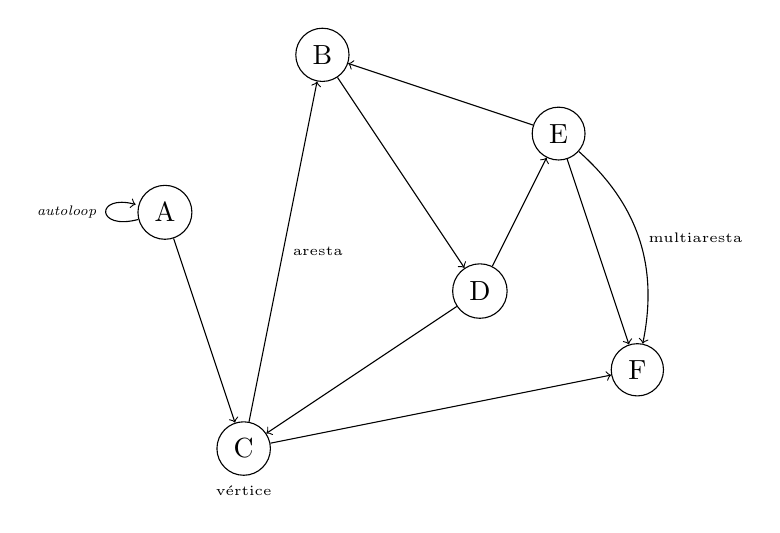
\begin{tikzpicture}
            \coordinate (A) at (0, 3);
            \coordinate (B) at (2, 5);
            \coordinate (C) at (1, 0);
            \coordinate (D) at (4, 2);
            \coordinate (E) at (5, 4);
            \coordinate (F) at (6, 1);

            \node[draw,circle] (A1) at (A) { A };
            \node[draw,circle] (B1) at (B) { B };
            \node[draw,circle] (C1) at (C) { C };
            \node[draw,circle] (D1) at (D) { D };
            \node[draw,circle] (E1) at (5, 4) { E };
            \node[draw,circle] (F1) at (6, 1) { F };

            \path (A1) edge[loop left] node[anchor=east] { \tiny \it autoloop } (A1);
            \draw[->] (A1) -- (C1);
            \draw[->] (C1) -- node[anchor=west] { \tiny aresta } (B1);
            \draw[->] (B1) -- (D1);
            \draw[->] (C1) -- (F1);
            \draw[->] (D1) -- (C1);
            \draw[->] (D1) -- (E1);
            \draw[->] (E1) -- (F1);
            \draw[->] (E1) -- (B1);
            \draw[->] (E1) to [bend left] node[anchor=west] { \tiny multiaresta } (F1);

            \node[anchor=north] at (C1.270) { \tiny vértice };
        \end{tikzpicture}

    \end{figure}

\end{frame}


